\chapter{BESCHREIBUNG DES ALGORITHMUS}
\label{see:art}

\section{ALGORITHMUS}

Der Algorithmus zur Berechnung des größten gemeinsamen Teilers von zwei ganzen Zahlen lautet wie folgt:

\vspace{\baselineskip}

\noindent Eingabe: zwei ganze Zahlen a und b.

\noindent Der Algorithmus verwendet den Euklidischen Algorithmus, um den größten gemeinsamen Teiler von zwei Zahlen zu berechnen. Daher müssen wir vor der Berechnung mit dem Euklidischen Algorithmus sicherstellen, dass die Eingaben gültige Werte sind, d.h. dass der Sonderfall der Berechnung des größten gemeinsamen Teilers ausgeschlossen ist.

\noindent Zunächst bestimmen wir den größten gemeinsamen Teiler zweier Zahlen im speziellen Eingabefall.

\noindent Im ersten Fall, wenn die beiden eingegebenen Zahlen einen oder mehrere Werte von 0 haben. Wenn a = 0, ist der Wert von b der größte gemeinsame Teiler der Zahlen a und b; Wenn b = 0, ist der Wert von a der größte gemeinsame Teiler der Zahlen a und b. 

\noindent Der zweite Fall, wenn die eingegebene Zahl eine negative Zahl ist. Wenn es eine negative Zahl gibt, müssen wir den absoluten Wert der negativen Zahl als Eingabe für die nachfolgenden Berechnungen nehmen. Wenn zum Beispiel a = -7 ist, muss der Wert von a in 7 geändert werden.

\noindent Nachdem die Eingabedaten verarbeitet wurden, wird hier der Euklidische Algorithmus verwendet, um ihren größten gemeinsamen Teiler zu berechnen.

\vspace{\baselineskip}

\noindent Der klassische euklidische Algorithmus berechnet den größten gemeinsamen Teiler, indem er nach einem gemeinsamen „Maß“ für die Längen zweier Linien sucht\cite*{lambacher}. Bei diesem Algorithmus muss der kleinere der beiden Werte vom größeren Wert abgezogen werden, bis das Ergebnis kleiner als der kleinere Wert ist. Das neue Ergebnis wird dann verwendet, um den vorherigen kleineren Wert zu ersetzen, und der kleinere Wert wird verwendet, um den vorherigen größeren Wert zu ersetzen. Danach wird der Algorithmus weiter angewandt.

\noindent Wenn die Differenz zwischen den beiden Eingabewerten 0 ist, wird die Berechnung beendet. Der Eingangswert ist dann der größte gemeinsame Teiler der beiden Eingänge. Andernfalls wiederholt man diesen Algorithmus.

\noindent In der Praxis kann der euklidische Algorithmus verwendet werden, um einige Probleme im Zusammenhang mit Modulo-Operationen zu lösen, wie z. B. die Berechnung von modulo-inversen Elementen und die Berechnung von Kongruenzgleichungen.

\section{PROGRAMMABLAUF}

In Abbildung 2.1 ist der Ablauf des Algorithmus dargestellt. Der Algorithmus verwendet zunächst zwei Beurteilungen, um die Möglichkeit auszuschließen, dass die eingegebene Zahl Null ist. Wenn in diesem Fall ein Eingang mit dem Wert 0 auftritt, wird der andere Eingangswert direkt als Ausgang verwendet. Dann verwendet er zwei weitere Beurteilungen, um mit Eingabewerten umzugehen, bei denen die Eingabe negativ ist. Nun wird das gleiche Register verwendet, um die ursprünglichen Daten mit den verarbeiteten Daten zu überschreiben. Dadurch wird die Verwendung von Registern reduziert.

\vspace{\baselineskip}

\noindent Nach den vier Beurteilungen wird dann der euklidische Algorithmus verwendet, um den größten gemeinsamen Teiler der beiden Eingaben zu berechnen. Bei diesem Algorithmus wird vor jeder Berechnung eine Beurteilung vorgenommen, um die Größe der beiden Eingabewerte jedes Mal zu vergleichen. Jedes Mal wird der größere Wert verwendet, um den kleineren Wert zu subtrahieren, und das Ergebnis der Berechnung wird durch den größeren Wert ersetzt. Da die Werte vor und nach dem Ersetzen im selben Register stehen, ist die Logik jeder Runde nahezu gleich. Dadurch wird die Komplexität des Logikentwurfs erheblich vereinfacht. Es spart auch die Verwendung von Registern.
 
\vspace{\baselineskip}

\begin{figure}[!htb]
  \centering
  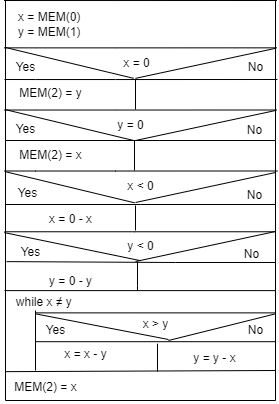
\includegraphics[width=0.5\textwidth]{images/ablaufplan.png}
  \caption[Programmablaufplan]{Programmablaufplan}
  \label{fig:ablaufplan}
\end{figure}



\cleardoublepage

